\documentclass[answers]{exam}
%\documentclass{exam}

\usepackage{xeCJK}
\usepackage{zhnumber}
\usepackage{graphicx}
\usepackage{hyperref}
\usepackage{amsmath}
\usepackage{booktabs}
\usepackage{enumerate}
\usepackage{amsmath}
\usepackage{appendix}
\usepackage{float}
\usepackage{color}


\pagestyle{headandfoot}
\firstpageheadrule
\firstpageheader{南京大学}{数字信号处理}{习题集一}
\runningheader{南京大学}
{数字信号处理}
{习题集一}
\runningheadrule
\firstpagefooter{}{第\thepage\ 页(共\numpages 页)}{}
\runningfooter{}{第\thepage\ 页(共\numpages 页)}{}

% no box for solutions
% \unframedsolutions

\setlength\linefillheight{.5in}

% \renewcommand{\solutiontitle}{\noindent\textbf{答:}}
\renewcommand{\solutiontitle}{\noindent\textbf{解:}\par\noindent}

\renewcommand{\thequestion}{\zhnum{question}}
\renewcommand{\questionlabel}{\thequestion .}
\renewcommand{\thepartno}{\arabic{partno}}
\renewcommand{\partlabel}{\thepartno .}


\begin{document}
\Large

\begin{questions}

\question 给出下列各时间函数的波形图:
\begin{enumerate}[(1)]
	\item $f_1(t) = \sin(\omega t) \cdot u(t)$
	\item $f_2(t) = \sin\left[ \omega (t-t_0) \right] \cdot u(t)$
	\item $f_3(t) = \sin\left[ \omega (t) \right] \cdot u(t-t_0)$
	\item $f_4(t) = \sin\left[ \omega (t-t_0) \right] \cdot u(t-t_0)$
\end{enumerate}

\begin{solution}
	{\color{red} 本题绘图见最后一页附录A}\\
	(1)将$sint$将横坐标变为原来的$1/w$倍,去掉$x<0$的部分\\

	(2)将$sint$将横坐标变为原来的$1/w$倍,然后右移$t_0$个单位,去掉$x<0$的部分\\

	(3)将$sint$的横坐标变为原来的$1/w$倍,然后去掉$x<t_0$的部分\\

	(4)将$sint$将横坐标变为原来的$1/w$倍,然后右移$t_0$个单位,去掉$x<t_0$的部分\\
\end{solution}



\question 已知$f(5-2t)$的波形如图~\ref{fig:q2-1}所示,画出$f(t)$的波形图。
\begin{figure}
	\centering
	\includegraphics{pics/q2-que.pdf}
	\caption{$f(5-2t)$波形图} \label{fig:q2-1}
\end{figure}

\begin{solution}
	{\color{red} 本题绘图见最后一页附录B}\\
	$f(5-2t)$是由$f(t)$先沿y轴作180°反转,然后进行压缩,最后右移2.5个单位而来,故$f(t)$的图像如下:

\end{solution}



\question 分别求下列周期信号的周期$T$:
\begin{enumerate}[(1)]
	\item $\cos(10t)-\cos(30t)$
	\item $e^{j10t}$
	\item $\left[5 \sin(8t) \right]^2$
	\item $\sum_{n=0}^{\infty} (-1)^n \left[ u(t-nT) - u(t-nT-T) \right]$($n$为正整数)
\end{enumerate}

\begin{solution}
	(1)$cos(10t)$的周期$T_1=\frac{\pi}{5}$,$cos(30t)$的周期$T_2=\frac{\pi}{15}$,$T_1/T_2$为有理数,故$cos(10t)-cos(30t)$的周期
	为$T_1,T_2$的最小公倍数,即$T=\frac{\pi}{5}$\\

	(2)由欧拉公式,$e^{j10t}=cos(10t)+jsin(10t)$,故周期为$T=\frac{\pi}{5}$\\

	(3)$[5sin(8t)]^2=25sin^2(8t)$,由二倍角公式,\\
	$25sin^2(8t)=\frac{25}{2}(1-cos(16t))$,故周期$T=\frac{\pi}{8}$\\

	(4)令$f(t)=u(t-nT)-u(t-nT-T)$\\

	显然$f(t)\mbox{仅在}nT\leq t<nT+T$时值为1,其他时间为0\\

	对于$\sum_{n=0}^{\infty}(-1)^nf(t)$,对某个t其中只有一项非0\\

	当$t\in[0,T)$时,第0项为1,其余各项为0,信号值为1\\
	当$t\in[T,2T)$,第1项为-1,其余各项为0,信号值为-1\\
	类似的,有$t\in[2kT,(2k+1)T),k=0,1,2..$时,值为1\\
	$t\in[(2k+1)T,(2k+2)T),k=0,1,2..$时,值为-1\\
	故该信号周期为$2T$
\end{solution}



\question 应用冲激信号的抽样特性,求下列表示式的函数值:
\begin{enumerate}[(1)]
	\item $\int_{-\infty}^{\infty} f(t-t_0)\delta(t) dt$
	\item $\int_{-\infty}^{\infty} f(t_0-t)\delta(t) dt$
	\item $\int_{-\infty}^{\infty} \delta(t-t_0)u(t-\frac{t_0}{2}) dt$
	\item $\int_{-\infty}^{\infty} \delta(t-t_0)u(t-2t_0) dt$
	\item $\int_{-\infty}^{\infty} (e^{-t}+t)\delta(t+2) dt$
	\item $\int_{-\infty}^{\infty} (t+\sin t)\delta(t-\frac{\pi}{6}) dt$
	\item $\int_{-\infty}^{\infty} e^{-j\omega t}\left[ \delta(t)-\delta(t-t_0)\right] dt$
\end{enumerate}

\begin{solution}
\begin{enumerate}[(1)]
	\item $f(-t_0)$
	\item $f(t_0)$
	\item $1$(值为$u(\frac{t_0}{2})$,此处假设$t_0>0$,第(4)问同)
	\item $0$(值为$u(-t_0)$)
	\item $e^2-2$
	\item $\pi/6+1/2$
	\item $1-e^{-jwt_0}$
\end{enumerate}
\end{solution}



\question 判断下列系统是否是线性的、时不变的、因果的,并说明理由:
\begin{enumerate}[(1)]
	\item $y(t) = \frac{d x(t)}{dt}$
	\item $y(t) = x(t)u(t)$
	\item $y(t) = \sin \left[x(t)\right]u(t)$
	\item $y(t) = x(1-t)$
	\item $y(t) = x(2t)$
	\item $y(t) = x^2(t)$
	\item $y(t) = \int_{-\infty}^t x(\tau) d\tau$
	\item $y(t) = \int_{-\infty}^{5t} x(\tau) d\tau$
\end{enumerate}

\begin{solution}
\begin{enumerate}[(1)]
	\item 线性:是,对于输入$\alpha x_1(t)+\beta x_2(t)$,系统的输出为$\alpha\frac{dx_1(t)}{dt}+\beta\frac{dx_2(t)}{dt}$\\
	时不变:是,因为$x(t-t_0)\rightarrow y(t-t_0)$\\
	因果的:是,响应不依赖于未来的信号\\
	\item 线性:是,对于输入$\alpha x_1(t)+\beta x_2(t)$,系统输出为$\alpha x_1(t)u(t)+\beta x_2(t)u(t)$\\
	时不变:不是,比如$x(t)$在$(-\infty,0)$上有值,输出与输入的关系随输入作用于系统的时间起点而改变\\
	因果的:是,响应不依赖于未来的信号\\
	\item 线性:不是,如$x(t)=t$,输入$2x(t)$,输出为$sin[2t]u(t)$而非$2sin(t)u(t)$\\
	时不变:不是,如$x(t)=t$时,输出与输入的关系随输入作用于系统的时间起点而改变\\
	因果的:是,响应不依赖于未来的信号\\
	\item 线性:是,输入$\alpha x_1(t)+\beta x_2(t)$,输出为$\alpha x_1(1-t)+\beta x_2(1-t)$\\
	时不变:是,因为$y(t)=x(1-t)\Rightarrow y(t-t_0)=x(1-(t-t_0))$\\
	因果的:不是,如$y(0)$依赖$x(1)$\\
	\item 线性:是,输入$\alpha x_1(t)+\beta x_2(t)$,输出为$\alpha x_1(2t)+\beta x_2(2t)$\\
	时不变:是,因为$y(t-t_0)=x(2(t-t_0))$\\
	因果的:不是,如$y(1)$依赖$x(2)$\\
	\item 线性:不是,如对于$x(t)=t$,输入$2x(t)$时输出为$4t^2$而非$2t^2$\\
	时不变:是,输出与输入的关系不会因为输入作用于系统的时间起点而改变\\
	因果的:是,响应不依赖于未来的信号\\
	\item 线性:是,积分具有线性性\\
	时不变:是,输出与输入的关系不会因为输入作用于系统的时间起点而改变\\
	因果的:是,响应不依赖于未来的信号\\
	\item 线性:是,积分具有线性性\\
	时不变:是,输出与输入的关系不会因为输入作用于系统的时间起点而改变\\
	因果的:不是,响应需要依赖未来的信号\\
\end{enumerate}
\end{solution}



\question 已知系统相应的齐次方程及其对应的$0_{+}$状态条件,求系统的零输入响应:
\begin{enumerate}[(1)]
	\item $\frac{d^2}{dt^2}y(t)+2\frac{d}{dt}y(t)+2y(t)=0$,给定:$y(0_{+})=1,y^{\prime}(0_{+})=2$
	\item $\frac{d^2}{dt^2}y(t)+2\frac{d}{dt}y(t)+y(t)=0$,给定:$y(0_{+})=1,y^{\prime}(0_{+})=2$
	\item $\frac{d^3}{dt^3}y(t)+2\frac{d^2}{dt^2}y(t)+\frac{d}{dt}y(t)=0$,给定:$y(0_{+})=y^{\prime}(0_{+})=0,y^{\prime\prime}(0_{+})=1$
\end{enumerate}

\begin{solution}
\begin{enumerate}[(1)]
	\item 特征方程为$\alpha^2+2\alpha+2=0$\\
	解得$\alpha_1=-1+j,\alpha_2=-1-j$\\
	故零输入响应\\
	$y_{zi}(t)=A_1e^{(-1+j)t}+A_2e^{(-1-j)t}=e^{-t}(A_1cost+A_2sint)$\\
	$y_{zi}(0_+)=1,y_{zi}'(0_+)=2$\\
	解得$A_1=1,A_2=3$\\
	所以零输入响应为$y_{zi}(t)=e^{-t}(cost+3sint)$\\
	\item 特征方程为$\alpha^2+2\alpha+1$\\
	解得$\alpha_1=\alpha_2=-1$\\
	故零输入响应\\
	$y_{zi}(t)=(A_1t+A_2)e^{-t}$\\
	代入$0_+$状态条件,解得$A_1=3,A_2=1$\\
	故零输入响应为$y_{zi}(t)=(3t+1)e^{-t}$\\
	\item 特征方程为$\alpha^3+2\alpha^2+\alpha=0$\\
	解得$\alpha_1=0,\alpha_2=\alpha_3=-1$\\
	故零输入响应\\
	$y_{zi}(t)=(A_1t+A_2)e^{-t}+A_3$\\
	代入$0_+$状态条件,解得$A_1=A_2=-1,A_3=1$\\
	故零输入响应$y_{zi}(t)=(-t-1)e^{-t}+1$\\
\end{enumerate}
\end{solution}



\question 求下列各个函数$x_1(t)$与$x_2(t)$的卷积$x_1(t)\ast x_2(t)$:
\begin{enumerate}[(1)]
	\item $x_1(t)=u(t),x_2(t)=e^{-at}u(t)$
	\item $x_1(t)=\delta(t),x_2(t)=\cos (\omega t + 45^{\circ})$
	\item $x_1(t)=(1+t)\left[u(t)-u(t-1)\right],x_2(t)=u(t-1)-u(t-2)$
	\item $x_1(t)=\cos(\omega t),x_2(t)=\delta(t+1)-\delta(t-1)$
	\item $x_1(t)=e^{-at}u(t),x_2(t)=(\sin t)u(t)$
\end{enumerate}

\begin{solution}
	$x_1(t)*x_2(t)=\int_{-\infty}^{\infty}x_1(\tau)x_2(t-\tau)d\tau$\\

	(1)$x_1(t)*x_2(t)=\int_{-\infty}^{\infty}u(\tau)e^{-a(t-\tau)}u(t-\tau)d\tau$\\
	$
=    \begin{cases}
        0\ t<0 \\
        \frac{1}{a}-\frac{1}{a}e^{-at}\  t\geq 0
    \end{cases}
$
\\

	(2)$x_1(t)*x_2(t)=\int_{-\infty}^{\infty}\delta(\tau)cos(w(t-\tau)+45°)d\tau$\\
	$=cos(wt+45°)$\\

	(3)$x_1(t)*x_2(t)=\int_{-\infty}^{\infty}(1+\tau)[u(\tau)-u(\tau-1)][u(t-\tau-1)-u(t-\tau-2)]d\tau$\\
	当$0\leq\tau<1$并且$t-1\leq\tau< t-2$时,卷积才不为0,故卷积结果如下:\\
	$
=    \begin{cases}
        0\ t<1\mbox{或者}t>3\\
        \frac{1}{2}t^2-\frac{1}{2}\  1\leq t<2\\
		-\frac{1}{2}t^2+t+\frac{3}{2}\ 2\leq t\leq3
    \end{cases}
$
\\

	(4)$x_1(t)*x_2(t)=\int_{-\infty}^{\infty}cos(w\tau)[\delta(t-\tau+1)-\delta(t-\tau-1)]d\tau$\\
	$=cos(w(t+1))-cos(w(t-1))$\\

	(5)$x_1(t)*x_2(t)=\int_{-\infty}^{\infty}e^{-a\tau}u(\tau)sin(t-\tau)u(t-\tau)d\tau$\\
	$
=    \begin{cases}
        0\ t<0 \\
        \frac{e^{-at}-cost+asint}{1+a^2}\  t\geq 0
    \end{cases}
$
\\	
\end{solution}



\question 设$x[n]=\delta[n]+2\delta[n-1]-\delta[n-3]$和$h[n]=2\delta[n+1]+2\delta[n-1]$,计算下列各卷积:
\begin{enumerate}[(1)]
	\item $y_1[n]=x[n]\ast h[n]$
	\item $y_2[n]=x[n+2]\ast h[n]$
	\item $y_3[n]=x[n]\ast h[n+2]$
\end{enumerate}

\begin{solution}
	$x[n]*h[n]=\sum_{k=-\infty}^{\infty}x[k]h[n-k]$\\

	(1)$y_1[n]=\sum_{k=-\infty}^{\infty}(\delta[k]+2\delta[k-1]-\delta[k-3])(2\delta[n-k+1]+2\delta[n-k-1])$\\
	
	$=\sum_{k=-\infty}^{\infty}(2\delta[k]\delta[n-k+1]+2\delta[k]\delta[n-k-1]+4\delta[k-1]\delta[n-k+1]$\\
	
	$+4\delta[k-1]\delta[n-k-1]-2\delta[k-3]\delta[n-k+1]-2\delta[k-3]\delta[n-k-1])$\\

	$=-2\delta[n-4]+2\delta[n-2]+2\delta[n-1]+4\delta[n]+2\delta[n+1]$\\

	$
=    \begin{cases}
        -2\ n=4\\
		2\ n=1,2,-1\\
		4\ n=0\\
		0\ \mbox{其他}
    \end{cases}
$\\

	(2)$y_2[n]=y_1[n+2]$\\

	$=-2\delta[n-2]+2\delta[n]+2\delta[n+1]+4\delta[n+2]+2\delta[n+3]$\\

	$
=    \begin{cases}
        -2\ n=2\\
		2\ n=-3,0,-1\\
		4\ n=-2\\
		0\ \mbox{其他}
    \end{cases}
$\\
	(3)

	$
y_3[n]=    \begin{cases}
        -2\ n=6\\
		2\ n=3,1,4\\
		4\ n=2\\
		0\ \mbox{其他}
    \end{cases}
$\\
\end{solution}



\question 已知输入$x[n]$和单位脉冲响应为$x[n]=\left(\frac{1}{2}\right)^{n-2}u[n-2]$,$h[n]=u[n+2]$,求输出$y[n]=x[n]\ast h[n]$,并画出$y[n]$。

\begin{solution}
	{\color{red} 本题绘图见最后一页附录C}\\
	$x[n]*h[n]=\sum_{k=-\infty}^{\infty}x[k]h[n-k]$\\

	故$y[n]=\sum_{k=-\infty}^{\infty}(\frac{1}{2})^{k-2}u[k-2]u[n-k+2]$\\

	$=\sum_{k=2}^{n+2}(\frac{1}{2})^{k-2}$\\

	$=2-(\frac{1}{2})^n(n\in N)$\\

	当$n\in N_-$时,$x[n]*h[n]=0$\\

\end{solution} 



\begin{figure}
	\centering
	\includegraphics[width=0.7\textwidth]{pics/q10.pdf}
	\caption{系统$S_1$和$S_2$的级联} \label{fig:q10-1}
\end{figure}
\question 考虑如图\ref{fig:q10-1}所示的两个系统$S_1$和$S_2$的级联,其中$S_1$为因果LTI,$\omega[n]=\frac{1}{2}\omega[n-1]+x[n]$,$S_2$为因果LTI,$y[n]=\alpha y[n-1]+\beta \omega[n]$。$x[n]$与$y[n]$的关系由下面的差分方程给出:$y[n]=-\frac{1}{8}y[n-2]+\frac{3}{4}y[n-1]+x[n]$。
\begin{enumerate}[(1)]
	\item 求$\alpha$和$\beta$
	\item 给出$S_1$和$S_2$级联后的单位脉冲响应
\end{enumerate}

\begin{solution}
\begin{enumerate}[(1)]
	\item $y[n]=-\frac{1}{8}y[n-2]+\frac{3}{4}y[n-1]+x[n]$\\
	$\rightarrow y[n]-\frac{1}{4}y[n-1]=\frac{1}{2}y[n-1]-\frac{1}{8}y[n-2]+x[n]$\\
	$\rightarrow (y[n]-\frac{1}{4}y[n-1])-\frac{1}{2}(y[n-1]-\frac{1}{4}y[n-2])=x[n]$\\

	考虑两个系统有$w[n]-\frac{1}{2}w[n-1]=x[n]$和$y[n]-\alpha y[n-1]=\beta w[n]$\\
	故$\alpha=\frac{1}{4},\beta=1$

	\item 单位脉冲响应为两个系统的单位脉冲响应的卷积,故分别计算$S_1,S_2$的单位脉冲响应\\
	对于$S_1$,有$h_1[n]=\frac{1}{2}h_1[n-1]+\delta[n]$\\
	用递推法求解\\
	$$
	h_1[0]-\frac{1}{2}h_1[-1]=1$$
	\\$$
	h_1[1]=\frac{1}{2}h_1[0]$$\\$$
	...
	$$\\
	解得$h_1[n]=(\frac{1}{2})^nu(n)$\\

	对于$S_2$,有$h_2[n]=-\frac{1}{8}h_2[n-2]+\frac{3}{4}h_2[n-1]+\delta[n]$\\
	类似的可以用递推法解得$h_2[n]=(\frac{1}{4})^nu(n)$\\
	故级联后的单位脉冲响应为:\\
	$h_1[n]*h_2[n]=\sum_{k=-\infty}^{\infty}h_1[k]h_2[n-k]$\\
	$=\sum_{k=0}^{n}(\frac{1}{2})^{2n-k}=[2(\frac{1}{4})^n-(\frac{1}{8})^n]u(n)$
\end{enumerate}
\end{solution}






\end{questions}

\newpage

\begin{appendices}
\section{第一题图片}

\begin{figure}[htbp]
	\centering
    \includegraphics[width=10cm,height=7cm]{pics/p1-1.jpg}
	\caption{第(1)问}
\end{figure}

\begin{figure}[htbp]
	\centering
    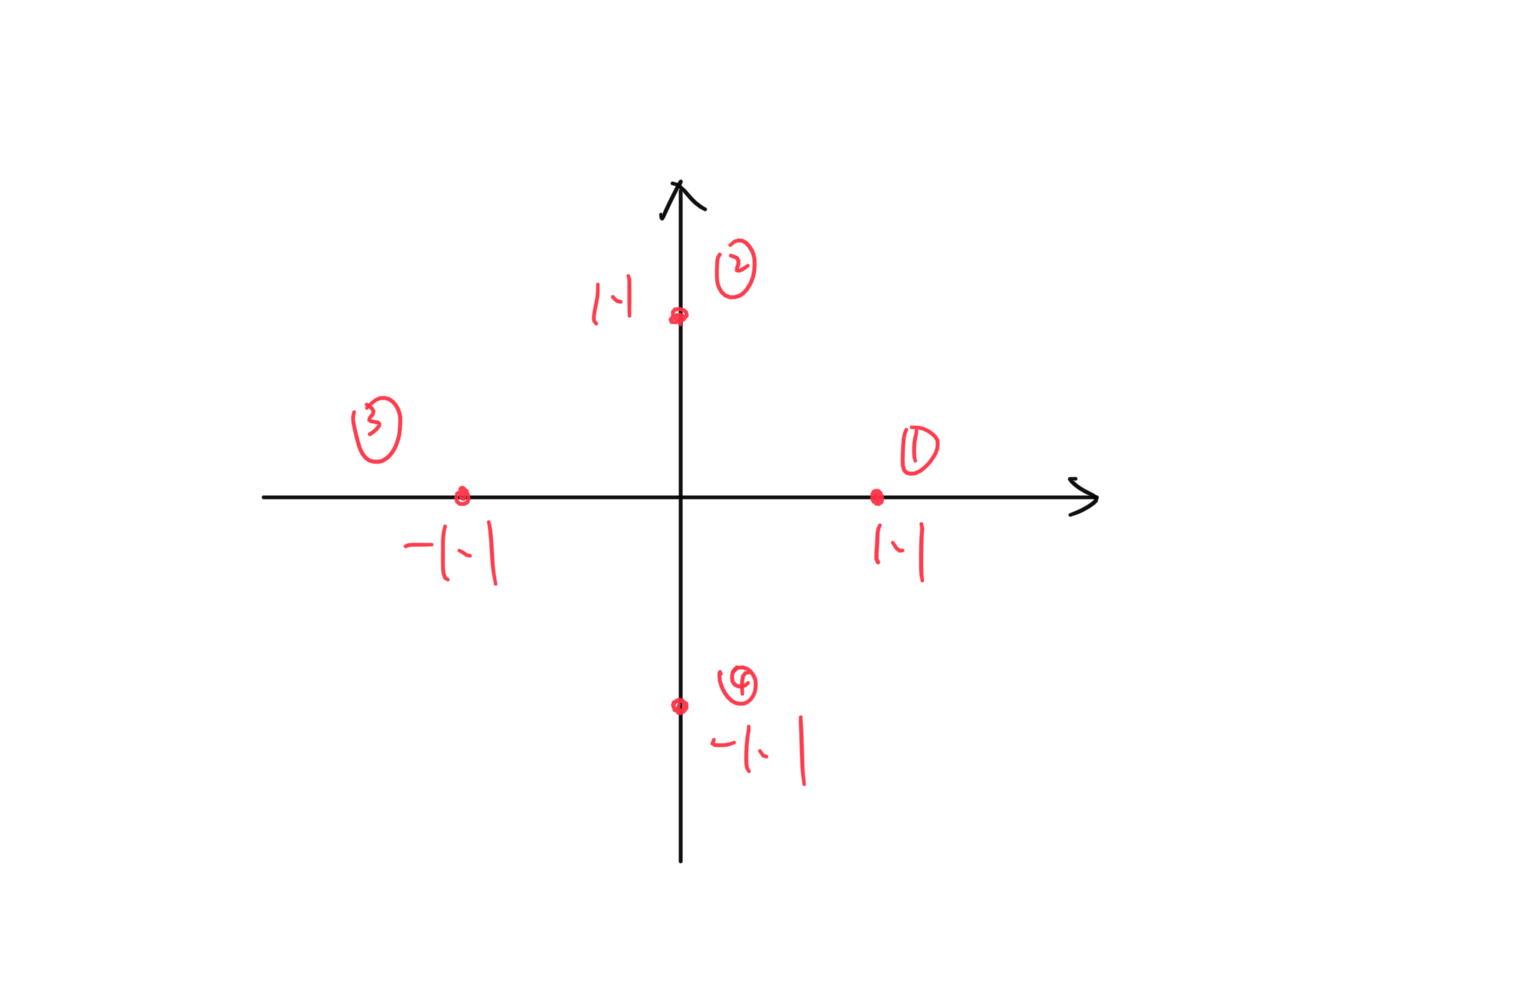
\includegraphics[width=10cm,height=7cm]{pics/p1-2.jpg}
	\caption{第(2)问}
\end{figure}

\newpage
\begin{figure}[h]
	\centering
    \includegraphics[width=10cm,height=7cm]{pics/p1-3.jpg}
	\caption{第(3)问}
\end{figure}

\begin{figure}[h]
	\centering
    \includegraphics[width=10cm,height=7cm]{pics/p1-4.jpg}
	\caption{第(4)问}
\end{figure}

\newpage
\section{第二题图片}
\begin{figure}[htbp]
    \includegraphics[width=15cm]{pics/p2.PNG}
	\caption{第二题}
\end{figure}

\newpage
\section{第九题图片}
\begin{figure}[htbp]
    \includegraphics[width=15cm]{pics/p9.png}
	\caption{第九题}
\end{figure}

\end{appendices}
\end{document}